\documentclass[11pt, a4paper, oneside]{report}
\usepackage{mathtools}
\usepackage{amsfonts}
\usepackage{minted}
\usepackage{booktabs}
\usepackage[UKenglish]{babel}
\usepackage[en-GB,showdow]{datetime2}
\usepackage{csquotes}
\usepackage{hyperref}
\usepackage{imakeidx} \makeindex
\usepackage[
sorting=none,
hyperref=true,
backend=biber,
style=numeric,
backref=true
]{biblatex}
\addbibresource{references.bib}
\usepackage{todonotes}
\usepackage{pdfpages}
\usepackage{glossaries} \makeglossaries
\usepackage{graphicx}
\usepackage{framed}
\usepackage{dsfont}
\usepackage{caption}
\usepackage{parskip}



\newglossaryentry{term}{ name={term}, description={``a
    word or expression that has a precise meaning in some uses or is
    peculiar to a science, art, profession, or
    subject'\autocite{dictionary:_term_defin_term} --- here text
    analysts have capitalised on the generalisation of ``term'to
    include subcomponents or aggregations of words} }




\begin{document}

% \frontmatter
\begin{titlepage}
  \centering
  \vspace*{2.5cm}
  {\Huge Text Analytics}\\
  \vspace{1.5cm}
  {\Large Jason Peter Cairns}\\
  \vspace{1.5cm}
  Supervised by Chris Wild\\
  \vspace{1.5cm}
  \begin{figure}[H]
    \centering
    
\includegraphics[scale=0.4]{img/logo.jpg}
  \end{figure}
  \vspace{1cm}
  Bachelor of Science (Honours)\\
  Department of Statistics\\
  The University of Auckland\\
  New Zealand
\end{titlepage}

\listoftodos

% \begin{abstract}

% \end{abstract}

\chapter*{Acknowledgements}
\label{cha:acknowledgements}

\tableofcontents
\addcontentsline{toc}{chapter}{Listings}
\renewcommand\listoflistingscaption{List of source codes}
\listoflistings
\addcontentsline{toc}{chapter}{Tables}
\listoftables
\addcontentsline{toc}{chapter}{Figures}
\listoffigures

% \mainmatter
\chapter{Introduction}
\label{cha:introduction}

\section{Intention}
\label{sec:intention}

Text Analytics serves to glean insight from a body of text. Within the
broad category of text analytics, we seek to answer questions about
what the text is communicating, what is felt about it, and how this
information is structured. In this dissertation, we demonstrate the
creation of a user-friendly program to perform text analytics
functions using modern R with the Shiny web application framework. In
a literate style, we illustrate top-down the structure of such a
program, as well as the data structures and computational processes
that have established their value for such a program.\todo{should this
  be an abstract?}
  
\section{Background: Text Analytics (incl. examples)}
\label{sec:backgr-text-analyt}

\todo{common functions: sentiment, summarisation, scoring}
\todo{Existing Systems}
\todo{current issues}

\section{Background: inZight}
\label{sec:background:-inzight}
\todo{What iNZight is - capabilities, popularity, etc.}
\todo{how our program fits in - shiny, inzight lite etc.}

\section{Literature Review (existing packages in R)}
\label{sec:liter-revi-exist}

\todo{Copy over from notes, flesh out a bit}
\todo{Praise tidytext book, complain about the package}

\section{Scope of work}
\label{sec:scope-work}

\todo{types of text that we can work with: novels, free response data etc.}
\todo{discuss limitations placed: not going into linguistic territory etc.}

\chapter{Text Analytics Prolusion}
\label{cha:text-analyt-backgr}

\section{overview}
\label{sec:overview}

\todo{Explain broadness of term}
\todo{compile glossary from terms here}
\todo{Areas of text analytics in a data science framework}
\todo{what we have done}
\todo{what we haven't done}

\section{terms}
\label{sec:terms}
\gls{term}
\todo{terms and their centrality}
\todo{generalisation: n-grams, sentences etc.}

\section{Historical Background}
\label{sec:hist-backgr}

\todo{computer science vs statistics - reflection in data science}

\section{Processing}
\label{sec:processing}

\todo{why process}
\todo{stopwords, lemmatisation etc.}
\todo{modelling vs db joins - more info in notes}

\section{scores \& statistics}
\label{sec:statistics}

\todo{why compute scores \& statistics}
\todo{scoring - tf-idf, word count}
\todo{Suggestions for further research - more on the statistics of words}
\todo{recount the book of John text analysis}

\section{Sentiment}
\label{sec:sentiment}

\todo{why sentiment}
\todo{Process of sentiment}
\todo{sentiment modelling vs db joins}
\todo{our implementation and why}
\todo{reviews}
\todo{issues}

\section{Summarisation}
\label{sec:summarisation}

\todo{why compute summarisations}
\todo{lexrank, textrank - include notes on lexrank}
\todo{other methods}
\todo{reddit bot example}

\section{what we didn't do (yet)}
\label{sec:what-we-didnt}

\todo{topic modelling}
\todo{Term correlation}
\todo{modelling based on linguistic features}

\section{Visualisation}
\label{sec:visualisation-1}

\todo{talk about score vs structure}
\todo{complain about tag clouds}
\todo{talk about ggpage}
\todo{discuss our experimentations with some alternative visualisations}
\chapter{Program Structure \& Development}
\label{cha:program-structure}

\todo{why R}
\todo{Why Shiny}
\todo{why tidyverse}
\todo{Git}
\todo{possible future: datatables, futures, etc.}
\todo{why functional}
\todo{Why lossless data}

\section{Program Architecture}
\label{sec:program-architecture-1}

\todo{Why structure it like it has been}
\todo{make graph of architecture}
\todo{Describe package and package creation}
\todo{following three sections copy and paste from the notes - buffing up as necessary}
\todo{include screenshots}

\section{Import}
\label{sec:import}

\section{Insight}
\label{sec:insight}

\section{Visualisation}
\label{sec:visualisation}

\section{User Interface}
\label{sec:user-interface}

\chapter{Conclusion}
\label{cha:conclusion}

\section{Summary}
\label{sec:summary}

\todo{summarise successes}
\todo{summarise failures}
\todo{general thoughts on the topic}

\section{Recommendations}
\label{sec:recommendations}

\todo{educational potential of text analytics}



\chapter{Appendix}
\label{cha:appendix}

The following pages are a copy of the documentation for the R package
created as a part of this dissertation. They were automatically
generated through the Roxygen2 system.

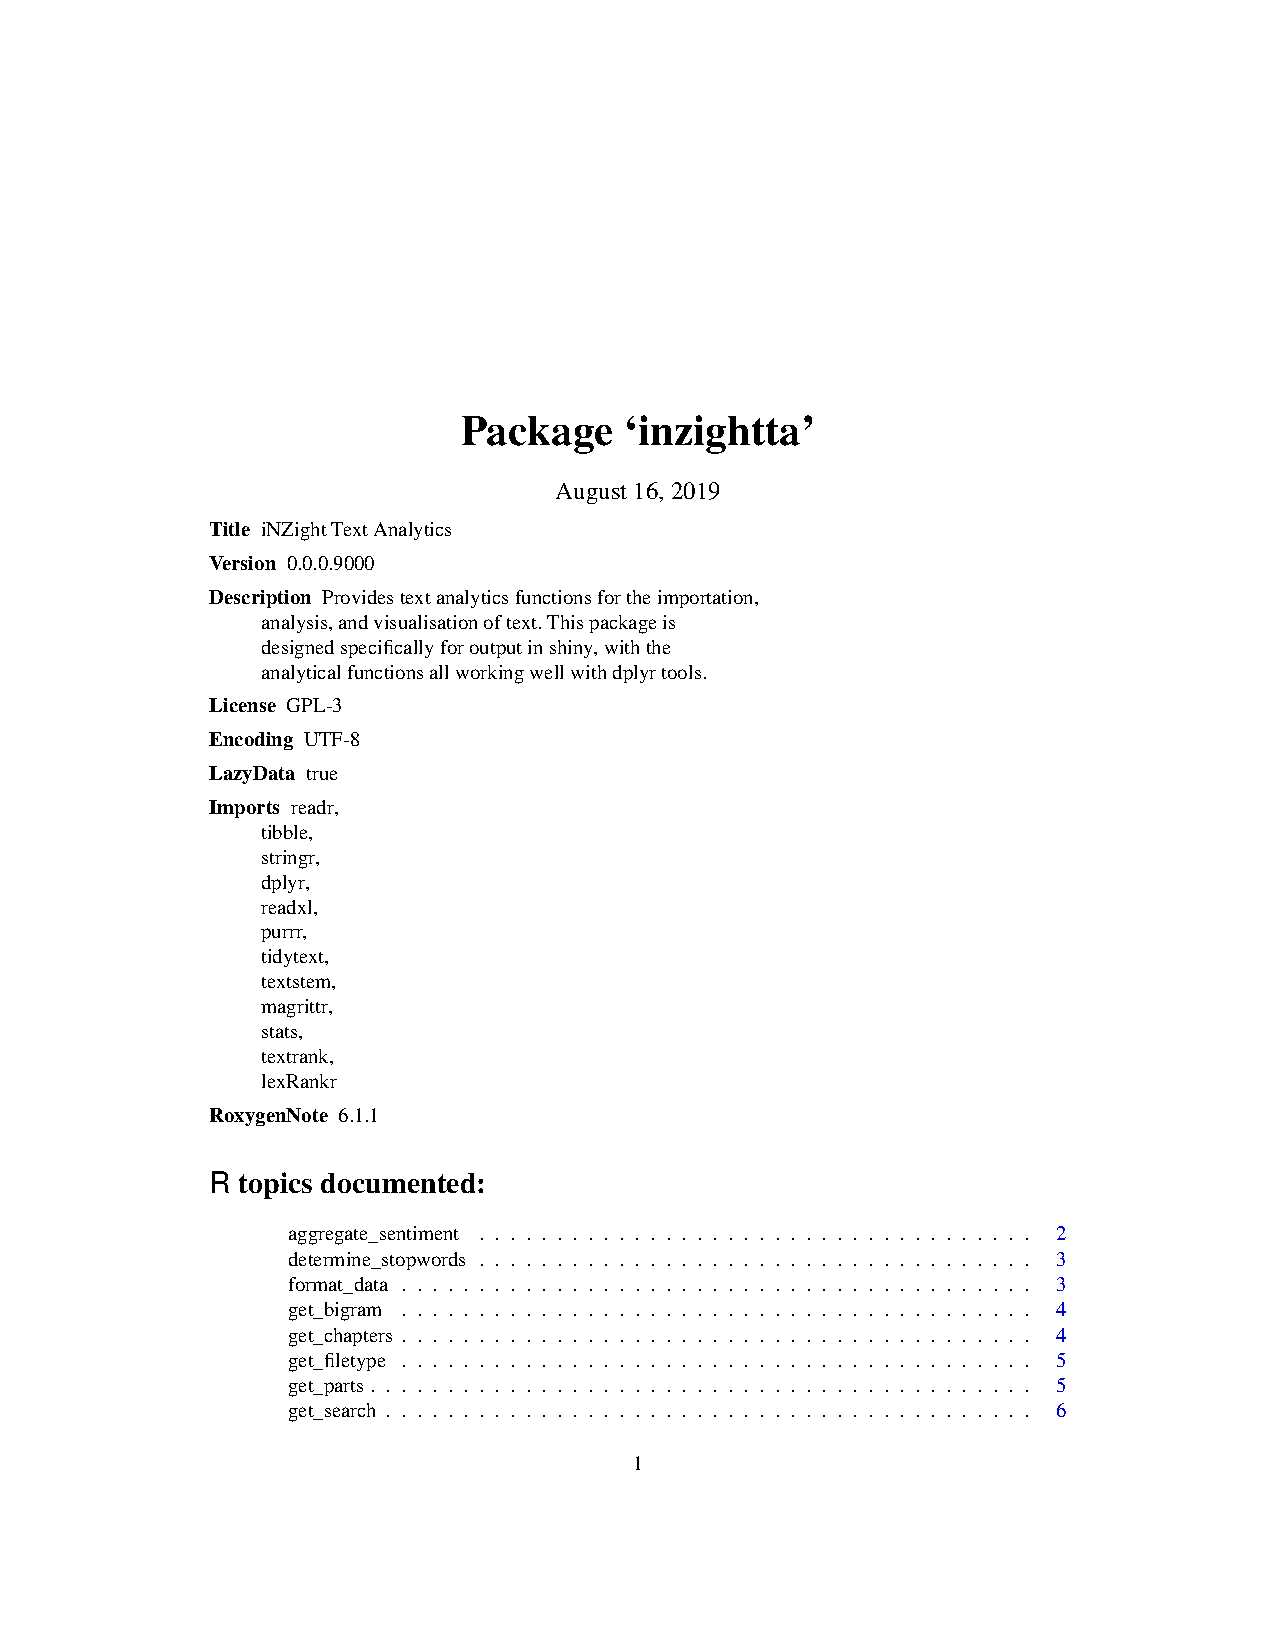
\includepdf[pages=-]{img/inzightta_manual.pdf}

% \backmatter
\addcontentsline{toc}{chapter}{Glossary}
\printglossaries
\addcontentsline{toc}{chapter}{Index}
\printindex
\addcontentsline{toc}{chapter}{Bibliography}
\printbibliography
\end{document}

% \begin{listing}[ht]
% \inputminted[
% frame=lines,
% framesep=2mm,
% fontsize=\footnotesize,
% linenos
% ]{R}{src/table.R}
% \caption{Example Code}
% \label{lst:test}
% \end{listing}

% \begin{table}[ht]
%   \centering
%   \input{src/output_table}
%   \caption{test table}
%   \label{tab:test}
% \end{table}